%% This is file `elsarticle-template-1-num.tex',
%%
%% Copyright 2009 Elsevier Ltd
%%
%% This file is part of the 'Elsarticle Bundle'.
%% ---------------------------------------------
%%
%% It may be distributed under the conditions of the LaTeX Project Public
%% License, either version 1.2 of this license or (at your option) any
%% later version.  The latest version of this license is in
%%    http://www.latex-project.org/lppl.txt
%% and version 1.2 or later is part of all distributions of LaTeX
%% version 1999/12/01 or later.
%%
%% Template article for Elsevier's document class `elsarticle'
%% with numbered style bibliographic references
%%
%% $Id: elsarticle-template-1-num.tex 149 2009-10-08 05:01:15Z rishi $
%% $URL: http://lenova.river-valley.com/svn/elsbst/trunk/elsarticle-template-1-num.tex $
%%
\documentclass[preprint,12pt]{elsarticle}

%% Use the option review to obtain double line spacing
%% \documentclass[preprint,review,12pt]{elsarticle}

%% Use the options 1p,twocolumn; 3p; 3p,twocolumn; 5p; or 5p,twocolumn
%% for a journal layout:
%% \documentclass[final,1p,times]{elsarticle}
%% \documentclass[final,1p,times,twocolumn]{elsarticle}
%% \documentclass[final,3p,times]{elsarticle}
%% \documentclass[final,3p,times,twocolumn]{elsarticle}
%% \documentclass[final,5p,times]{elsarticle}
%% \documentclass[final,5p,times,twocolumn]{elsarticle}

%% The graphicx package provides the includegraphics command.
\usepackage{graphicx}
\usepackage[colorlinks,linkcolor=red]{hyperref}
%% The amssymb package provides various useful mathematical symbols
\usepackage{amssymb}
\usepackage{caption}
\usepackage{graphicx} % Required for including pictures
\usepackage{titlesec}
\usepackage{float} % Allows putting an [H] in \begin{figure} to specify the exact location of the figure
%% The amsthm package provides extended theorem environments
%% \usepackage{amsthm}

%% The lineno packages adds line numbers. Start line numbering with
%% \begin{linenumbers}, end it with \end{linenumbers}. Or switch it on
%% for the whole article with \linenumbers after \end{frontmatter}.
\usepackage{lineno}

%% natbib.sty is loaded by default. However, natbib options can be
%% provided with \biboptions{...} command. Following options are
%% valid:

%%   round  -  round parentheses are used (default)
%%   square -  square brackets are used   [option]
%%   curly  -  curly braces are used      {option}
%%   angle  -  angle brackets are used    <option>
%%   semicolon  -  multiple citations separated by semi-colon
%%   colon  - same as semicolon, an earlier confusion
%%   comma  -  separated by comma
%%   numbers-  selects numerical citations
%%   super  -  numerical citations as superscripts
%%   sort   -  sorts multiple citations according to order in ref. list
%%   sort&compress   -  like sort, but also compresses numerical citations
%%   compress - compresses without sorting
%%
%% \biboptions{comma,round}

% \biboptions{}

\journal{Journal Name}

\begin{document}

\begin{frontmatter}

%% Title, authors and addresses

\title{The Predicting Power of Investor Emotion}

%% use the tnoteref command within \title for footnotes;
%% use the tnotetext command for the associated footnote;
%% use the fnref command within \author or \address for footnotes;
%% use the fntext command for the associated footnote;
%% use the corref command within \author for corresponding author footnotes;
%% use the cortext command for the associated footnote;
%% use the ead command for the email address,
%% and the form \ead[url] for the home page:
%%
%% \title{Title\tnoteref{label1}}
%% \tnotetext[label1]{}
%% \author{Name\corref{cor1}\fnref{label2}}
%% \ead{email address}
%% \ead[url]{home page}
%% \fntext[label2]{}
%% \cortext[cor1]{}
%% \address{Address\fnref{label3}}
%% \fntext[label3]{}


%% use optional labels to link authors explicitly to addresses:
%% \author[label1,label2]{<author name>}
%% \address[label1]{<address>}
%% \address[label2]{<address>}

%\author{John Smith}

\address{California, United States}

\begin{abstract}
%% Text of abstract
Though recently many studies have been conducted to validate the relationship between investor's emotion and the stock price changes. Exploiting the relationship for predicting purpose has driven way less attentions than it deserve. In this paper, we summarized the prevaling methologies conducted in anazlying the relationship between stock changes and investor emotion and some important conclusions. Based upon those conclusions, we exploited the predictability of the investor emotion on abnormal financial returns via LSTM Nerual Network. Out result indicate that the investor emotion has tremendous advantages in predicting the financial returns....
\end{abstract}

\begin{keyword}
Science \sep Publication \sep Complicated
%% keywords here, in the form: keyword \sep keyword

%% MSC codes here, in the form: \MSC code \sep code
%% or \MSC[2008] code \sep code (2000 is the default)

\end{keyword}

\end{frontmatter}

%%
%% Start line numbering here if you want
%%


%% main text
\section{Review of Current Methodlogies}
Someone did blablabla....

\section{Predicting the "Abnormal Returns"}
\subsection{Motivation for Analysis}
$$R_t=\alpha_t+\beta*R_m$$

	As... has claimed, the CAPM model is great in decomposing the finacial returns into the normal one (related to the market) and the "abnormal one" (related to individual events). Many investors have profitted from concentrating on predicting the abnormal return (by implementing the alpha strategy). Successively Predicing the abnormal return then could have tremendous meaning in beating the market.
    Though the investment strategies differ from each other, they all reach to one final destination of making transaction and for all the transactions made, there are emotion drove behind those decisions. Thus exploiting the investor emotion to predict the returns doesn't contradict with any validated investment (example: foundament analysis, technical analysis or quantitative analysis). 
    If the predicting is accurate, then it is possible to further decompose the abnormal returns into the emotion category and thus rewrite the pricing formular of individual stocks.
\subsection{Data Gathering} 
\subsubsection{Emotion Data}
	Doing emotion analysis from text is taxing and it involves a lot of subjectivities. As.... has claim, the perfect emotion classifier doesn't exist and thus, in our analysis, we utilized the emotion data classifed by ... In the paper of...., the classification has been accredited 75\% accuracy and is sufficient to validate the predictability of investor emotion.
   	Emotion data Can be download from
    \href{http://kt.ijs.si/data/Twitter_sentiment_DJIA30}{data}.\\
\subsubsection{Returns Data}
	As metioned before, we concentrated on predicting the abnormal return. Thus we first decompose the return of individual stocks via CAPM model.
    $$R_t=\alpha_t+\beta*R_m$$
    
    The $\alpha$ value is the abnormal return that we are attempting to predict because the individual stock emotion is more likely to affect the alpha value than the market as a whole.\\
    So we first construct a moving average for the daily series of the alpha return of individual stocks. It is important to note that predicting the moving average of alpha value is equivalent to predicting the alpha return on specfic day because suppose at today, we know tomorrow's alpha moving average then by having the access to the histrocial alpha data, we can actually solve for the next day's specifc alpha returns.\\
    After computing the 30 days moving average, we compare the path of the 30 days positive emotion ratio moving average and the 30 days' moving average alpha.\\
    \begin{figure}[H]
	\centering
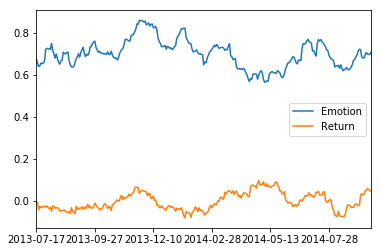
\includegraphics[width=3in]{1.png}
	\caption{Comparison}
\end{figure}
    
    As we can see, there are some of the relationships between the emotion and the alpha value, and we further calculate the correlation coefficient between them:\\
 \begin{figure}[H]
	\centering
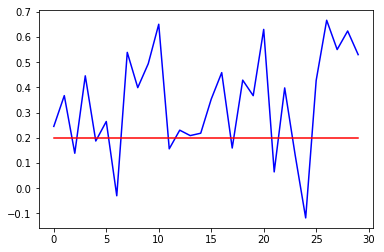
\includegraphics[width=3in]{2.png}
	\caption{Correlation}
\end{figure}
    For the 30 stocks we chosen, most of them has the correlation above 0.2.\\
\subsection{LSTM---predicting Model}
	In the Machine Learning field, LSTM has been proven its effectiveness in predicting time series data. Here we adopted the same model to predict the alpha returns.\\
    The input values are three variables: Total number of positive emotion, total number of negative emotion, total number of neutral emotions.\\
    The out put value is the 30 days moving average alpha value of returns.\\
    The predicting result is:\\
\begin{figure}[H]
	\centering
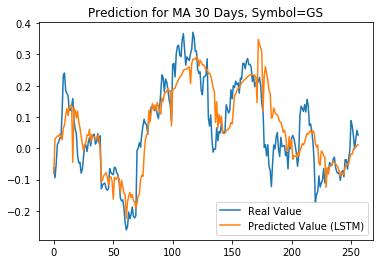
\includegraphics[width=3in]{GS__.png}
	\caption{Prediction of LSTM}
\end{figure}
    We can see that we have achieved very promising result in exploiting the predictability of investor's emotion.
\section{Discussion}
\subsection{Overfitting}
	We used drop out neural network to see that if we drop certain neuros in the training how does the result differ from the original ones....

\section{Conclusion}
    It has predicting power...
    
   
    
   	
    
    
    
    
%% The Appendices part is started with the command \appendix;
%% appendix sections are then done as normal sections
%% \appendix

%% \section{}
%% \label{}

%% References
%%
%% Following citation commands can be used in the body text:
%% Usage of \cite is as follows:
%%   \cite{key}          ==>>  [#]
%%   \cite[chap. 2]{key} ==>>  [#, chap. 2]
%%   \citet{key}         ==>>  Author [#]

%% References with bibTeX database:

\bibliographystyle{model1-num-names}
\bibliography{sample.bib}

%% Authors are advised to submit their bibtex database files. They are
%% requested to list a bibtex style file in the manuscript if they do
%% not want to use model1-num-names.bst.

%% References without bibTeX database:

% \begin{thebibliography}{00}

%% \bibitem must have the following form:
%%   \bibitem{key}...
%%

% \bibitem{}

% \end{thebibliography}


\end{document}

%%
%% End of file `elsarticle-template-1-num.tex'.
